\documentclass[10pt,a4paper]{scrartcl}
\usepackage[utf8]{inputenc}
\usepackage[T1]{fontenc}
\usepackage[ngerman]{babel}
\usepackage{microtype, multicol, marginnote, bera, parskip}
\usepackage{listings, amsmath, amssymb, graphicx, tikz, epic}
\usepackage{stmaryrd} %for lightning arrow
\usepackage{pstricks, pst-node, pst-tree, pdflscape}
\usepackage[babel=true]{csquotes}
\usepackage{placeins}
\tolerance=2000
\setcounter{secnumdepth}{0}
\usepackage[inner=2.5cm,outer=2.5cm,top=1.5cm,bottom=1.5cm,includeheadfoot]{geometry}
\newcommand{\subExercise}[1]{\vspace{1em} \noindent{\bf #1)}}
\author{Michael Mardaus \and Andrey Tyukin}
\title{
\includegraphics[scale=0.2]{../logo_schriftzug}\\
Technische Informatik: Submission 4}

\begin{document}

\maketitle

\section*{Exercise 4.1 (Decoder Fulladder)}

We can construct a fulladder from a 3-8-Decoder and 
two OR-Gates

\vspace{1em}
\begin{figure}[h]
  \centering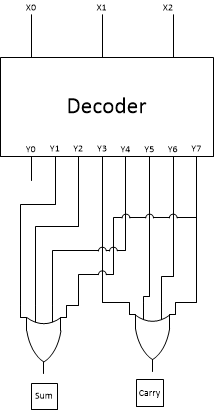
\includegraphics[width=4cm]{images/fulladder.png}
  \caption{Fulladder}
\end{figure}
\vspace{1em}

\FloatBarrier
% Exercise 2.2
\section*{Exercise 2 ()}
open

\section*{Exercise 3: (Racing and Beting)}
open

\end{document}
